\documentclass[11pt,a4paper]{article}

\usepackage[margin=1.1in]{geometry}
\usepackage{graphicx}
\usepackage{amsmath}
\usepackage{amssymb}
\usepackage{booktabs}
\usepackage{array}
\usepackage{enumitem}
\usepackage{setspace}
\usepackage{url}
\usepackage[hidelinks]{hyperref}
\usepackage{eso-pic}
\usepackage{tikz}

% ------------------------------------------------------------------ Formal page border on every page
\AddToShipoutPictureBG{%
  \begin{tikzpicture}[remember picture, overlay]
    \draw[black, line width=0.8pt]
      ([xshift=0.45in,yshift=-0.45in]current page.north west) rectangle
      ([xshift=-0.45in,yshift=0.45in]current page.south east);
  \end{tikzpicture}%
}

\begin{document}

% ---------------------------------------------------------------- Title page
\begin{titlepage}
\centering
{\large\bfseries DEPARTMENT OF ARTIFICIAL INTELLIGENCE AND DATA SCIENCE\par}
\vspace{0.2cm}
{\large Amrita Vishwa Vidyapeetham, Delhi NCR, Faridabad\par}
\vspace{0.5cm}
\rule{0.55\linewidth}{0.8pt}\par
\vspace{1.8cm}

{\Huge\bfseries Inferno\par}
\vspace{0.35cm}
{\Large A Fused Int4 CUDA Kernel and an MPI-Coordinated\\
Adaptive Serving Stack for Large Language Model Inference\par}
\vspace{0.6cm}
{\large\bfseries CUDA kernel~$\cdot$~MPI request router~$\cdot$~rigorous GPU benchmarking\par}
\vspace{0.8cm}
{\large\itshape Mid-Semester Project Report\par}
\vspace{2.0cm}

{\large B.Tech (AIDS), UG-III (V Semester)\par}
{\large High-Performance Computing Project\par}
\vspace{1.3cm}

{\large
\begin{tabular}{ll}
Likhith & DL.AI.U4AID24117 \\[2pt]
Karthikeya & DL.AI.U4AID24020 \\[2pt]
Sandeep & DL.AI.U4AID24143 \\[2pt]
A.\ Karthik & DL.AI.U4AID24104 \\
\end{tabular}
\par}

\vfill
{\large Submitted to: [Faculty Guide Name]\par}
\vspace{0.4cm}
{\large \today\par}
\end{titlepage}

% -------------------------------------------------------------------- Abstract
\section*{Abstract}
Serving large language models (LLMs) quickly is, at its core, a memory-bandwidth problem, made harder by bursty
request traffic and the need to coordinate several GPU replicas at once. This report presents \textit{Inferno}, a
project built around three components: a hand-written, fused int4 CUDA kernel for the memory-bound decode step of
LLM inference; an MPI-coordinated request router that distributes requests across multiple pre-loaded model
replicas; and a load-aware adaptive controller that chooses between routing policies at runtime. The project is
organized around one guiding question: \emph{can a parallel, adaptive serving stack beat fixed configurations, and
why?} As instructed, this mid-semester report is limited to the Introduction, the Literature Review, and the
Proposed Methodology: it explains the problem in detail, surveys the prior work the project builds on, and describes
the complete design of the kernel, the router, and the experimental methodology used to evaluate them. The kernel,
its integration into the vLLM serving engine, the routing infrastructure, and the measurement harness are already
built and running on an NVIDIA RTX 4060 Laptop GPU (8~GB); the confirmatory measurement campaign, GPU-level
profiling, and a multi-GPU cloud evaluation are in progress, and the complete results will be presented in full by
the end of November 2026.

\vspace{0.25cm}
\noindent\textbf{Keywords:} LLM inference, CUDA, quantization, GPU kernels, MPI, parallel computing, benchmarking methodology.

\newpage
\tableofcontents
\newpage

\onehalfspacing

\section{Introduction}

\subsection{Motivation: The Memory Bandwidth Problem}
Autoregressive language models generate text one token at a time, and at every single decoding step the model must
read its \emph{entire} set of weights from GPU memory to produce just one new token. For the 1.5-billion-parameter
model used throughout this project (Qwen2.5-1.5B-Instruct), the FP16 weights occupy approximately 3.1~GB. The RTX~4060
Laptop GPU used for all experiments has a theoretical memory bandwidth of 256~GB/s. A simple back-of-envelope
calculation --- dividing the amount of data that must be read by how fast the GPU can read it --- gives an idealized
upper bound of roughly 83 tokens per second at batch size one, if generation were limited purely by reading weights
from memory. Our own measured FP16 baseline, 67 tokens per second, sits close to this bound, which is itself strong
evidence that at small batch sizes, decoding speed is governed primarily by \emph{how fast weights can be read from
memory}, not by how fast the GPU's arithmetic units can compute. This behaviour is a well-known pattern in
high-performance computing called the \emph{roofline} model of performance \cite{roofline}: when an operation performs
very little arithmetic per byte of data moved, its speed is capped by memory bandwidth rather than by compute
throughput. This is not true of every LLM workload --- processing a long prompt (prefill), or decoding with a very
large batch of requests at once, can instead be compute-bound --- but it is exactly the regime that matters most for
interactive, low-latency serving, which is what this project targets. The direct engineering consequence is that if
the model's weights can be stored in a smaller format, for example 4-bit integers (int4) instead of 16-bit floating
point, as produced by post-training quantization methods such as AWQ~\cite{awq} and GPTQ~\cite{gptq}, there are
roughly four times fewer bytes to read per token, and generation can potentially run proportionally faster ---
\emph{if} a kernel exists that can actually operate on this compact format without paying a tax elsewhere, as
demonstrated for batched inference by kernels such as Marlin~\cite{marlin}. Writing such a kernel, efficiently, for
this project's own single-sequence decode setting, is the first major piece of this project.

\subsection{Three Engineering Problems We Must Solve}
Beyond the memory-bandwidth problem itself, two further engineering problems compound it once a model is actually put
into production:
\begin{enumerate}[leftmargin=1.5em, itemsep=6pt]
  \item \textbf{Memory-bound decoding.} At small batch sizes, the speed of generating a token is often limited by the
        number of bytes that must be read from GPU memory rather than by how much arithmetic the GPU can perform.
        Smaller (int4) weights~\cite{awq,gptq} mean fewer bytes to read, and therefore a real opportunity for
        speedup, provided the kernel reading and using them is itself efficient~\cite{marlin}.
  \item \textbf{Bursty traffic and tail latency.} Production request traffic rarely arrives at a perfectly steady
        rate; it comes in bursts. Users experience the \emph{slowest} requests they personally send, not the average
        across all users, which is why serving systems are increasingly judged on tail (99th-percentile, or $p_{99}$)
        latency and \emph{goodput} rather than raw throughput alone~\cite{distserve,splitwise}, and must be evaluated
        under realistic, time-varying load rather than a single steady rate.
  \item \textbf{Coordinating replicas.} Serving at any meaningful scale requires running several copies (replicas) of
        the model at once~\cite{orca,vllm}, and incoming requests must be distributed among them through a
        coordination layer that itself adds as little overhead as possible.
\end{enumerate}

\subsection{Why This Is a High-Performance-Computing Problem}
Each of the three problems above maps naturally to a distinct parallel-computing technique, which is what makes this
fundamentally a High-Performance-Computing project rather than a purely machine-learning one. The decode step is a
matrix--vector product with billions of independent multiply-accumulate operations spread across output rows and
reduction elements; this is exactly the kind of fine-grained, regular data parallelism a GPU is built for, and it is
addressed in this project with a hand-written CUDA kernel (Section~\ref{sec:parallel}). Serving multiple independent
replicas, and routing independent requests among them, is a distributed-memory coordination problem, addressed with
an MPI-based dispatcher-and-worker architecture (Section~\ref{sec:parallel}). Finally, because performance claims
about parallel systems are notoriously easy to get wrong --- through measurement artefacts, caching effects, or
simply not measuring enough repetitions --- every experiment in this project is designed and analyzed with a
pre-specified, statistically paired protocol \cite{georges,hoefler} (Section~\ref{sec:rigor}).

\noindent\textbf{Research Question.} Can a parallel, adaptive serving stack beat fixed configurations --- and why, or
why not?

\medskip
\noindent\textbf{Relevance to High-Performance Computing.} Three elements of this project map directly onto
established HPC concerns: (i)~\emph{GPU/CUDA} --- billions of independent multiply-add operations, addressed with
fine-grained data parallelism; (ii)~\emph{MPI} --- coordinating many independent, in-flight requests across separate
model replicas; and (iii)~\emph{rigorous benchmarking} --- so that any speed claim this project makes can actually be
trusted.

\subsection{Objectives of the Project}
The project is organized around five measurable objectives:
\begin{enumerate}[leftmargin=1.6em, itemsep=8pt]
  \item \textbf{Design a fused int4 CUDA kernel} that reaches at least 85\% of the GPU's theoretical DRAM
        bandwidth for batch-1 decoding, measured against Marlin~\cite{marlin} as the state-of-the-art baseline, so
        that quantization actually translates into real speed rather than being offset by inefficient implementation.
  \item \textbf{Integrate that kernel into a production serving engine (vLLM)~\cite{vllm}} and measure real,
        end-to-end decode throughput, rather than only a stand-alone microbenchmark that may not reflect real serving
        conditions.
  \item \textbf{Pre-specify and test a hypothesis (H1)} that a load- and length-aware adaptive router achieves lower
        tail latency than the strongest fixed configuration, at no worse throughput, and to report the outcome
        honestly whichever way it goes.
  \item \textbf{Design and evaluate an MPI-based request router}, measuring its coordination overhead and how it is
        expected to scale as more replicas and nodes are added.
  \item \textbf{Conduct the entire study with a reproducible, statistically defensible methodology}, in which every
        number that is ever reported is generated programmatically from raw measurement files, never transcribed by
        hand.
\end{enumerate}

\subsection{Scope of This Report}
This is a \emph{mid-semester} report, and as requested its scope is limited to the Introduction, the Literature
Review, and the Proposed Methodology: the problem this project addresses, the prior work it builds on, and the
complete design of the CUDA kernel, the MPI-based router, and the experimental methodology used to evaluate them.
Sections~\ref{sec:parallel}--\ref{sec:rigor} describe work that is \textbf{already built and running}. Results are not
presented in this report; the confirmatory measurement campaign, GPU-level profiler (Nsight Compute) confirmation of
the kernel's design choices, a tensor-core kernel variant for larger batch sizes, and a multi-GPU cloud evaluation are
in progress, and the complete results will be presented in the final report and evaluation at the end of November
2026.

\section{Literature Review}
\label{sec:lit}
This project builds on four threads of prior work, spanning serving-system design, disaggregated deployment,
model quantization, and rigorous performance measurement.

\subsection{Continuous and Paged Serving}
Orca~\cite{orca} introduced \emph{iteration-level} (continuous) batching for transformer serving: rather than
batching requests at the level of whole requests, the scheduler admits and retires individual requests between
decoding iterations, so a finished request does not have to wait for every other request in its batch to finish, and
a newly arrived request does not have to wait for the whole batch to complete before joining in. This substantially
improves throughput over naive request-level batching. vLLM~\cite{vllm} addressed the memory side of the same
problem with \emph{PagedAttention}, which stores each request's key--value (KV) cache in small, non-contiguous,
fixed-size blocks, much like how an operating system pages memory, instead of one large contiguous allocation. This
reduces wasted memory from fragmentation and lets many more requests be served in parallel with the same GPU memory.
vLLM is used as the serving engine throughout this project, precisely because it already solves these two problems
well.

\subsection{Disaggregated Serving}
DistServe~\cite{distserve} and Splitwise~\cite{splitwise} observe that the two phases of LLM inference have very
different resource profiles: processing an incoming prompt (prefill) is compute-bound, while generating tokens one
at a time (decode) is memory-bound, as established in Section~\ref{sec:lit} above this subsection. Both systems
place these two phases on separate GPUs to avoid one interfering with the other, and both optimize for
\emph{goodput} --- the rate of requests that are served within an acceptable latency, rather than raw throughput
alone --- a metric this project also adopts when evaluating routing policies. Their central, and most relevant,
premise is that co-locating heterogeneous work on shared hardware causes measurable interference. This premise is
the direct motivation for this project's own adaptive-routing evaluation, in which multiple model replicas are made
to share a single physical GPU, precisely so that this kind of interference can be observed, measured, and explained
rather than assumed away.

\subsection{Quantization and Quantized Kernels}
AWQ~\cite{awq} and GPTQ~\cite{gptq} are two widely used post-training quantization methods that compress model
weights down to 3--4 bits per parameter while keeping accuracy loss small. AWQ does this by identifying a small
number of weight channels that matter disproportionately, guided by activation statistics, and protecting them from
aggressive rounding; GPTQ instead uses an approximate second-order correction to choose each rounded weight so that
the overall error introduced into the layer's output is minimized. Marlin~\cite{marlin} is a family of highly
optimized, mixed-precision GPU kernels specifically built to run inference efficiently on 4-bit weights produced by
methods like these, and it is tuned in particular for batched, multi-sequence inference. Marlin is the direct
baseline this project's own hand-written kernel is designed against and measured against, both as a stand-alone
microbenchmark and once fully integrated inside vLLM.

\subsection{Rigorous Benchmarking Practice}
Hoefler and Belli~\cite{hoefler} survey common pitfalls in how parallel-computing performance is reported and give a
set of concrete guidelines for measuring and presenting results defensibly, including running enough repetitions,
reporting variability rather than a single number, and being explicit about what exactly was measured. Georges et
al.~\cite{georges} demonstrate, with real measurements on modern systems, that run-to-run performance
non-determinism can be large enough to make a single-run comparison between two systems statistically meaningless
without confidence intervals and repeated measurement. These two works directly motivate the paired,
repeated-measures experimental design and the statistical protocol this project adopts throughout, described fully
in Section~\ref{sec:rigor}.

\subsection{The Gap We Fill}
None of the four threads above combine all three of this project's concerns --- a hand-optimized quantized kernel, a
distributed request router, and a statistically rigorous evaluation --- on a single, resource-constrained GPU, and
none of them commit, in advance, to reporting a design idea as unsuccessful if the measurements do not support it.
This project studies the kernel, the router, and the statistics together, on shared hardware, and is designed from
the outset to report its findings honestly regardless of which way any given result turns out.

\subsection{How This Review Shaped Our Objectives}
The four threads surveyed above were not read for background alone; each one directly shaped a specific design
decision behind the five objectives listed in Section~1.4.
\begin{itemize}[leftmargin=1.4em, itemsep=6pt]
  \item Continuous and paged serving is the direct reason \textbf{vLLM} was chosen as the serving engine (Objective
        2), rather than building request scheduling and KV-cache management from scratch, which would have consumed
        effort without adding anything Orca and vLLM had not already solved well.
  \item Quantization and quantized-kernel research set both the \emph{storage format} our own kernel is built to
        decode --- the packed, group-wise int4 layout popularized by AWQ and GPTQ --- and the \emph{baseline},
        Marlin, that the kernel's design target of 85\% bandwidth is measured against (Objective 1).
  \item Disaggregated serving's central finding, that co-located heterogeneous work interferes on shared hardware,
        is the direct reason this project pre-specifies and tests a hypothesis about adaptive routing (Objective 3)
        instead of simply assuming an adaptive router would help.
  \item The rigorous-benchmarking literature is the direct source of this project's statistical methodology:
        paired tests, multiple-repetition designs, and a commitment to generating every reported number from raw
        data rather than by hand (Objective 5).
  \item None of the four threads addresses distributed coordination of replicas on constrained, single-machine
        hardware, which is why the request router in Objective 4 is built independently with MPI rather than adapted
        from any one paper above.
\end{itemize}
In short, the gap identified in Section~2.6 above --- that no existing work studies the kernel, the router, and the
statistics together --- is precisely the gap this project's five objectives are built to fill.

\section{Proposed Methodology}
\label{sec:method}

\subsection{System Workflow}
Figure~\ref{fig:architecture} shows the overall system, organized into three groups: inputs, the system under test,
and measurement and analysis.
\begin{enumerate}[leftmargin=1.6em, itemsep=6pt]
  \item \textbf{Workload generator.} Produces seeded request streams under three patterns --- steady (Poisson
        arrivals), bursty, and a mixed-length pattern combining short and long requests --- so that every pattern
        can be replayed exactly.
  \item \textbf{Open-loop client.} Sends every request at its scheduled arrival time, whether or not earlier
        requests have finished, and records time-to-first-token, time-per-output-token, and end-to-end latency. An
        open-loop client is used deliberately: a closed-loop client silently reduces its own offered load as the
        system slows down, which would hide exactly the queueing behaviour this project needs to measure.
  \item \textbf{Request router.} Decides which replica serves each request. This can be a fixed policy, a
        least-outstanding-requests HTTP baseline, the adaptive controller under test, or the MPI dispatcher
        (rank~0).
  \item \textbf{vLLM replicas.} A pool of resident, pre-loaded vLLM replicas --- a low-latency tier and a
        high-throughput tier --- sharing a single GPU.
  \item \textbf{Fused int4 CUDA kernel.} The heavy computational work inside decoding: decoding each packed 4-bit
        weight and using it immediately, described fully in Section~\ref{sec:parallel}.
  \item \textbf{Metrics and power.} Per-request latencies and GPU power draw are recorded continuously throughout
        every experiment.
  \item \textbf{Statistics.} A paired statistical protocol, described in Section~\ref{sec:rigor}, decides whether an
        observed difference between two policies is real or could plausibly be chance.
  \item \textbf{Report and dashboard.} All downstream analysis --- statistical tests, plots, and this report itself
        --- is a pure function of the recorded raw files, so every number is regenerable rather than transcribed by
        hand.
\end{enumerate}

\begin{figure}[!htb]
\centering
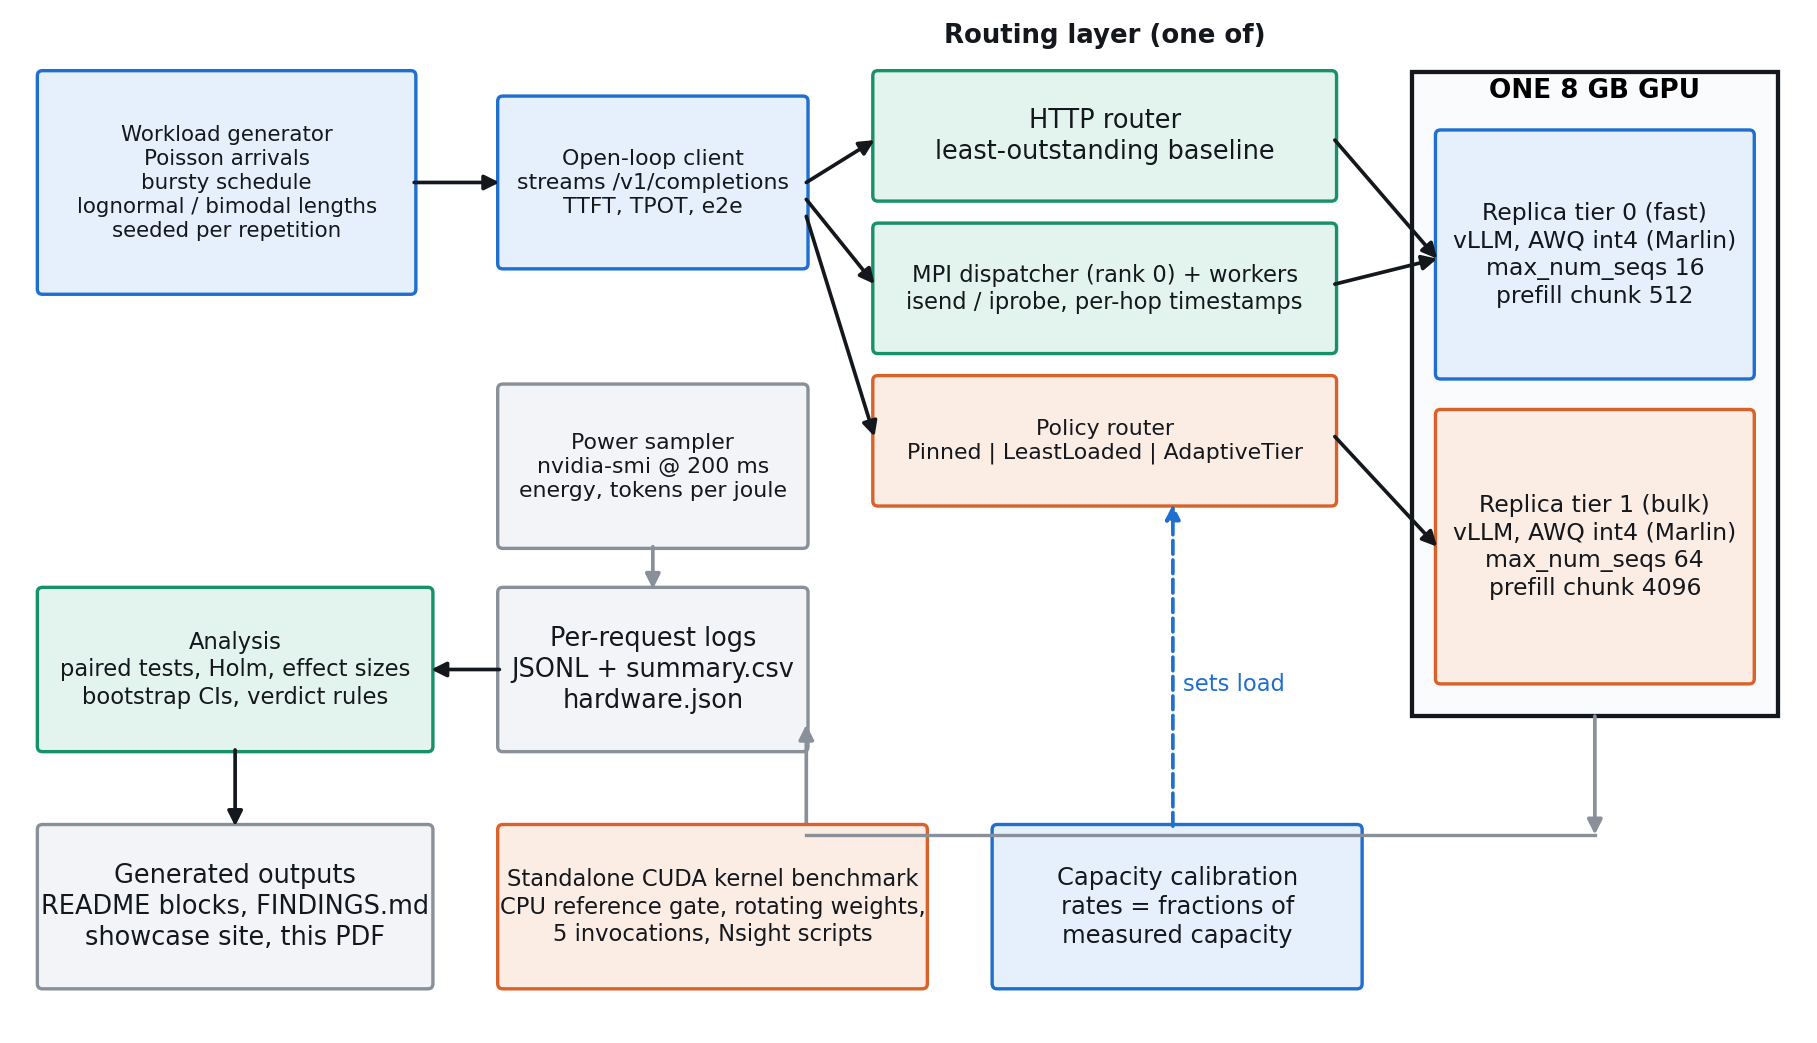
\includegraphics[width=0.92\linewidth]{figures/architecture.png}
\caption{System architecture: workload generation, routing, the resident replica pool on one GPU, and the
measurement/analysis pipeline.}
\label{fig:architecture}
\end{figure}

\noindent\textbf{Key Idea.} The \emph{same} seeded traffic is replayed through every policy being compared, so that
any difference in the outcome comes from the policy itself, not from random variation in the traffic each policy
happened to see.

\subsection{Parallelization Strategy}
\label{sec:parallel}
Table~\ref{tab:parallel} identifies the independent units of work at three distinct levels of the system, and the
parallel-computing framework used at each level, together with the reasoning behind that choice.

\begin{table}[!htb]
\caption{Parallelization strategy: independent tasks and framework justification at each level.}
\label{tab:parallel}
\centering
\small
\renewcommand{\arraystretch}{1.25}
\begin{tabular}{@{}>{\raggedright\arraybackslash}p{2.0cm}>{\raggedright\arraybackslash}p{4.0cm}>{\raggedright\arraybackslash}p{4.9cm}>{\raggedright\arraybackslash}p{4.9cm}@{}}
\toprule
\textbf{Level} & \textbf{Independent tasks} & \textbf{Parallel design} & \textbf{Framework \& justification} \\
\midrule
\textbf{Level 1} \newline CUDA \newline (inside one layer) &
Each output row of a matrix--vector product; each row further splits into independent 32-weight chunks. &
16 GPU threads (lanes) cooperate per output row; wide, coalesced memory loads; a fast warp-level reduction combines
partial sums. &
\textbf{CUDA.} This is fine-grained, regular data parallelism on a memory-bandwidth-bound task --- exactly the
regime a GPU's many concurrent memory pipelines are built for. \\
\addlinespace
\textbf{Level 2} \newline vLLM \newline (across users) &
Decode tokens belonging to different, independent user requests. &
Continuous (iteration-level) batching \cite{orca}; a decoded weight is reused across every concurrent request
before being discarded. &
\textbf{vLLM.} A mature, widely used serving engine already solves request-level scheduling and KV-cache management
well; re-implementing it would add no value, so it is used as-is and our kernel is integrated into it. \\
\addlinespace
\textbf{Level 3} \newline MPI \newline (across replicas) &
Whole, independent inference requests, each servable by any one of several model replicas. &
A rank-0 dispatcher process routes each request to a worker rank with a non-blocking send; each worker polls for new
work with a non-blocking probe and owns one replica connection. &
\textbf{MPI.} Requests are embarrassingly parallel across replicas, and MPI is a distributed-memory model: the same
dispatcher/worker code scales from one GPU to a multi-node cluster without modification, which the multi-GPU
evaluation planned for November requires. Measured one-way latency is approximately 2~microseconds for a small
control message. \\
\bottomrule
\end{tabular}
\end{table}

\noindent\textbf{Note.} MPI coordinates requests; it does not accelerate the GPU arithmetic. That acceleration is
entirely the responsibility of the CUDA kernel in Level~1. Two alternative frameworks were considered and rejected:
OpenMP, which parallelizes shared-memory CPU code and has no GPU execution model; and NCCL, which is designed for
collective communication of tensors between GPUs (for example in distributed training) rather than for routing
independent, heterogeneous requests. A plain HTTP router with a least-outstanding-requests policy is retained
throughout as the baseline against which the MPI router's overhead is measured.

Within Level~1, the kernel itself decodes each packed 4-bit weight directly into a fast on-chip register and
multiplies it immediately, instead of first converting the whole weight matrix back into a larger, full-precision
format and writing that copy back out to GPU memory. Avoiding that extra round trip to memory is what allows the
smaller int4 storage format to translate into real speed rather than being offset by wasted memory traffic
elsewhere. Every version of the kernel, on every layer shape it is run against, is checked for correctness against a
reference implementation before any timing measurement from it is trusted.

\subsection{Tools, Technologies and Experimental Setup}
\label{sec:rigor}

\subsubsection*{Hardware and Software Stack}
All experiments run on a single NVIDIA RTX~4060 Laptop GPU (8~GB) under WSL2 Ubuntu on a 16-core machine. GPU kernels
are written in CUDA~12.4, with cuBLAS used as the reference FP16 baseline; GPU-level profiling with Nsight Compute is
planned but pending, since it currently requires a Windows driver setting this project does not yet have access to
enable. The serving engine is vLLM~0.11 on PyTorch~2.8, with the project's own kernel registered as a custom
PyTorch operator so it can be swapped in transparently. Distributed coordination uses Open~MPI~5.0.10 with the
\texttt{mpi4py} bindings, and the planned multi-GPU evaluation will run on cloud infrastructure already provisioned
as Terraform configuration. All statistical analysis uses NumPy, SciPy, and pandas, and both the written report and
the project's live dashboard are generated automatically from the same underlying result files. The model used
throughout is Qwen2.5-1.5B-Instruct, evaluated in three precisions: FP16, GPTQ-Int8, and AWQ-Int4.

\subsubsection*{Experimental Design}
The kernel is evaluated on six real decoder-layer shapes drawn from Qwen2.5-1.5B and Llama-7B, with every kernel
version checked against a double-precision CPU reference before any timing run is trusted. The confirmatory serving
campaign evaluates four routing policies under three load patterns (steady, bursty, and mixed-length), with eight
repetitions of each combination, giving $4 \times 3 \times 8 = 96$ experimental runs of 75~seconds each. Offered
load is never guessed: a reference replica is first saturated to measure its maximum sustainable capacity, and every
experimental load level is then expressed as a calibrated fraction of that measured capacity --- for example, the
steady-load pattern is set to run at 60\% of measured capacity. The end-to-end study inside vLLM separately covers
five configurations at batch sizes from one to eight sequences, using CUDA-graph decode and three repeats per
configuration. Throughout, the metrics tracked are time-to-first-token, time-per-output-token, the 50th, 95th, and
99th percentile latencies, goodput, tokens per second, and tokens per joule of GPU energy. All workloads are seeded,
synthetic request streams rather than an external dataset, which means every run is exactly repeatable and no
licensing or availability concerns apply to the data used.

\subsubsection*{Statistical Rigor}
Within each repetition of the confirmatory campaign, every routing policy replays an \emph{identical}, seeded
request stream, so that any difference observed between policies is attributable to the policy itself and not to
random variation in the traffic it happened to see; the order in which policies are run within a repetition is
itself randomized, to cancel out any thermal drift on the GPU over the course of an experiment. The comparison
between the adaptive policy and the best fixed configuration uses a paired Student's $t$-test together with the
non-parametric Wilcoxon signed-rank test, and a result is only treated as statistically significant if both tests
agree, with a Holm correction applied for running the comparison across three separate load patterns. Eight
repetitions were chosen deliberately to give this combined test enough statistical headroom: with too few paired
repetitions, neither test can ever report a significant result, no matter how large the underlying effect actually
is, so eight was chosen with margin above the minimum that theory requires.

\begin{figure}[!htb]
\centering
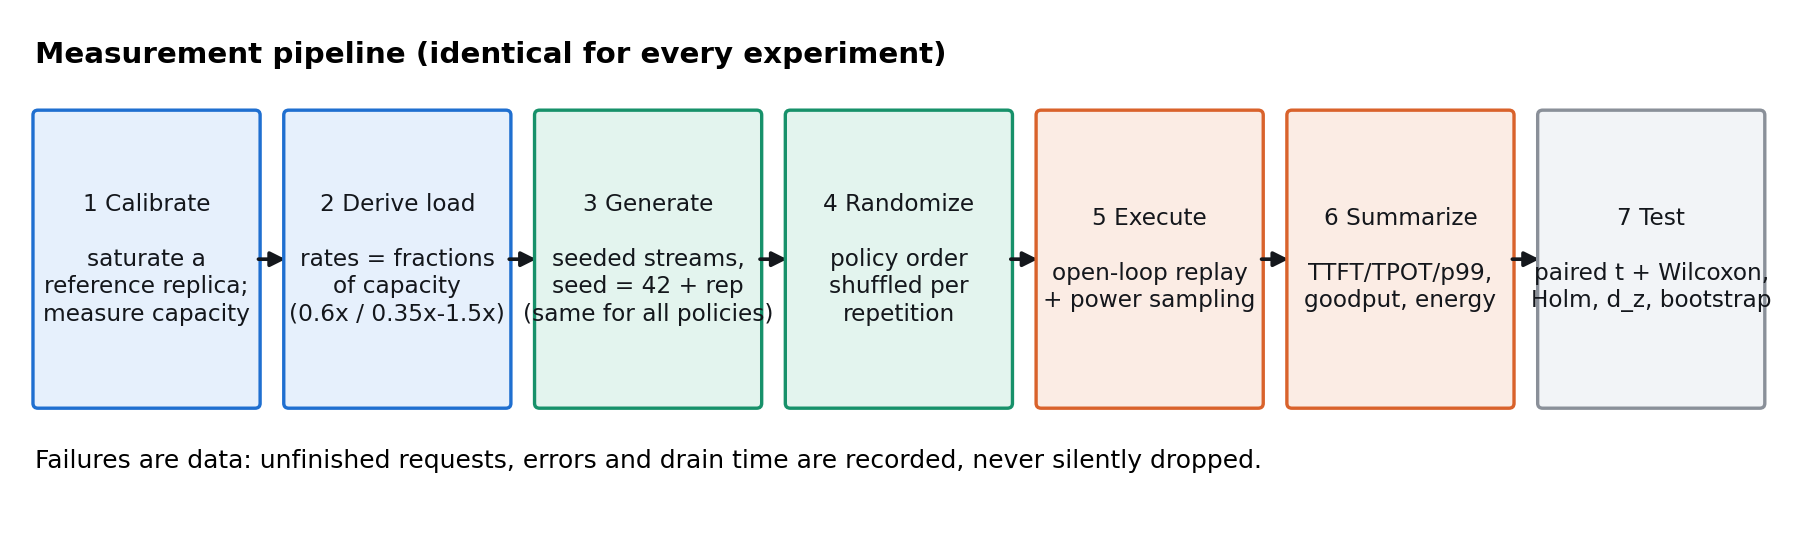
\includegraphics[width=0.92\linewidth]{figures/pipeline.png}
\caption{The measurement pipeline, applied identically to every experiment in this project.}
\label{fig:pipeline}
\end{figure}

\noindent\textbf{Reproducibility.} Same seed in, same result out, every time: no number in this project's report,
dashboard, or presentation is ever typed in by hand; every one of them is produced by the project's own analysis
scripts running on raw measurement files.

\begin{thebibliography}{00}
\bibitem{orca} G.-I.~Yu, J.~S.~Jeong, G.-W.~Kim, S.~Kim, and B.-G.~Chun, ``Orca: A distributed serving system for
transformer-based generative models,'' in \textit{Proc. USENIX OSDI}, 2022.
\bibitem{vllm} W.~Kwon, Z.~Li, S.~Zhuang, Y.~Sheng, L.~Zheng, C.~H.~Yu, J.~Gonzalez, H.~Zhang, and I.~Stoica,
``Efficient memory management for large language model serving with PagedAttention,'' in \textit{Proc. ACM SOSP},
2023.
\bibitem{distserve} Y.~Zhong, S.~Liu, J.~Chen, J.~Hu, Y.~Zhu, X.~Liu, X.~Jin, and H.~Zhang, ``DistServe:
Disaggregating prefill and decoding for goodput-optimized large language model serving,'' in \textit{Proc. USENIX
OSDI}, 2024.
\bibitem{splitwise} P.~Patel, E.~Choukse, C.~Zhang, A.~Shah, I.~Goiri, S.~Maleki, and R.~Bianchini, ``Splitwise:
Efficient generative LLM inference using phase splitting,'' in \textit{Proc. ACM/IEEE ISCA}, 2024.
\bibitem{awq} J.~Lin, J.~Tang, H.~Tang, S.~Yang, W.-M.~Chen, W.-C.~Wang, G.~Xiao, X.~Dang, C.~Gan, and S.~Han, ``AWQ:
Activation-aware weight quantization for LLM compression and acceleration,'' in \textit{Proc. MLSys}, 2024.
\bibitem{gptq} E.~Frantar, S.~Ashkboos, T.~Hoefler, and D.~Alistarh, ``GPTQ: Accurate post-training quantization for
generative pre-trained transformers,'' in \textit{Proc. ICLR}, 2023.
\bibitem{marlin} E.~Frantar, R.~L.~Castro, J.~Chen, T.~Hoefler, and D.~Alistarh, ``MARLIN: Mixed-precision
auto-regressive parallel inference on large language models,'' in \textit{Proc. ACM PPoPP}, 2025.
\bibitem{hoefler} T.~Hoefler and R.~Belli, ``Scientific benchmarking of parallel computing systems: Twelve ways to
tell the masses when reporting performance results,'' in \textit{Proc. SC}, 2015.
\bibitem{georges} A.~Georges, D.~Buytaert, and L.~Eeckhout, ``Statistically rigorous Java performance evaluation,''
in \textit{Proc. ACM OOPSLA}, 2007, pp.~57--76.
\bibitem{roofline} S.~Williams, A.~Waterman, and D.~Patterson, ``Roofline: An insightful visual performance model for
multicore architectures,'' \textit{Commun. ACM}, vol.~52, no.~4, pp.~65--76, 2009.
\end{thebibliography}

\end{document}
